%-------------------------------------------------------------------
% QUESTIONS First Principles
%-------------------------------------------------------------------
\begin{Exercise}[title={Differentiation from First Principles}, label=exFirstPrinciples]
	\Question Find the derivative of the function at the given value using the method of first principles.
	\begin{tasks}
		\task $f (x) =5 x^{2} +3 x -1$ at the number $2$%23
		\task $f (x) =1 -3 x^{2}$ at the number $2$%-12
		\task $f (x) =x^{4}$ at the number $1$, given $(x +h)^{4} =x^{4} +4 x^{3} h +6 x^{2} h^{2} +4 x h^{3} +h^{4}$%4
	\end{tasks}

{\hspace{-0.6cm}\textbf{Graphing Exercises}}	
\Question The graph of $f (x) =(x -1) (x +2) (x -3)$ is drawn below. On the same set of axes, sketch the graph of the derived function, $f^{ \prime } (x)$. What is the shape of the graph of the derived function?\\
\begin{center}
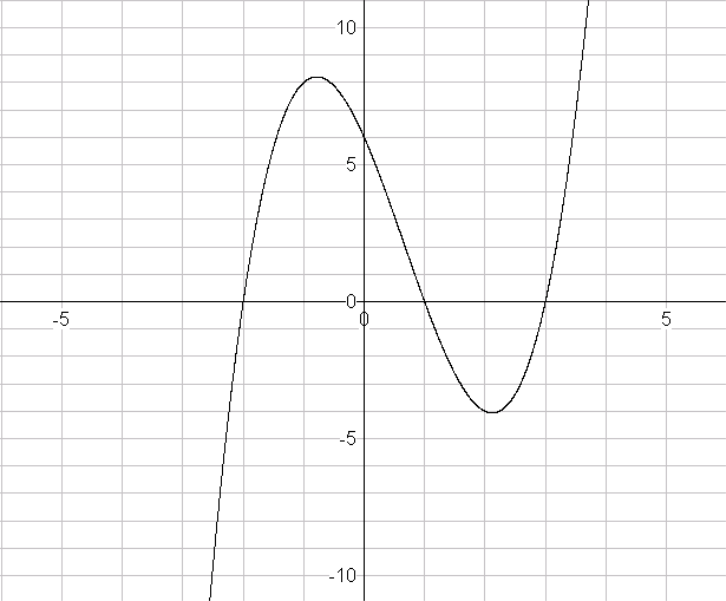
\includegraphics[width=12cm]{L4SZ2834}
\end{center}

%Use Desmos to plot the graph and compare to yours.
\Question The graph of $f (x) =(x +1) (x -1) (x -2) (x +3)$ is drawn below. On the same set of axes, sketch the graph of the derived function, $f^{ \prime } (x)\vspace{+0.500000cm}$ \\
\begin{center}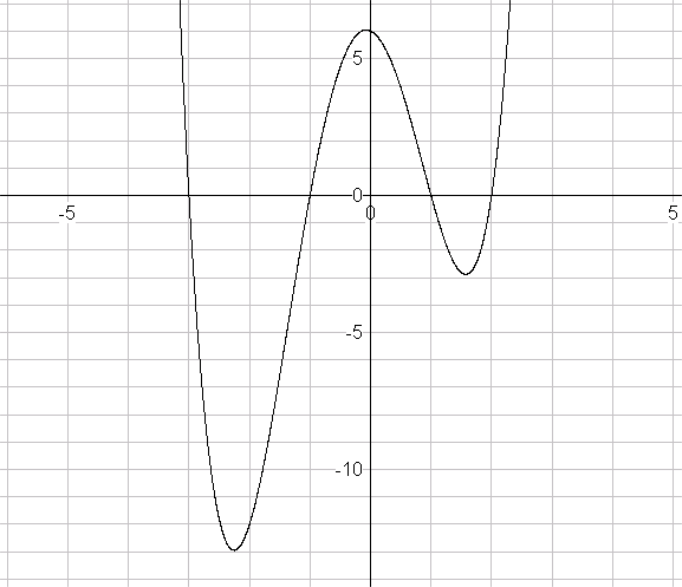
\includegraphics[width=12cm]{L4SZ2835}\end{center}
What is the order of $f (x)$? What is the order of $f^{ \prime } (x)$?%Use Desmos to check
\Question The graph of $f (x) =e^{x}$ is drawn below. On the same set of axes, sketch the graph of the derived function, $f^{ \prime } (x)\vspace{+0.500000cm}$ \\
\begin{center}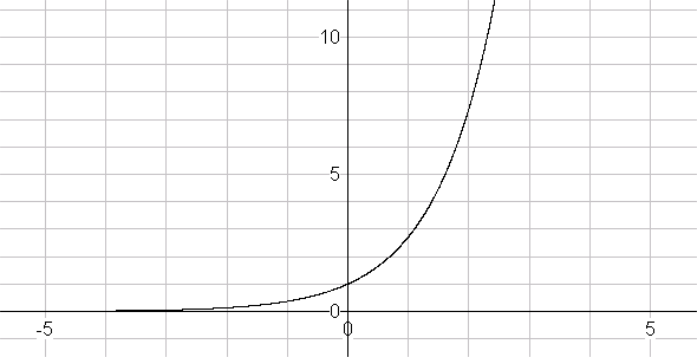
\includegraphics[width=13cm]{L4SZ2836}\end{center}
What is the shape of the graph of the derived function?	
\Question The graph of $f (x) =10 x^{2} e^{x} (x +1)$ is drawn below. On the same set of axes, sketch the graph of the derived function, $f^{ \prime } (x)\vspace{+0.500000cm}$ \\
\begin{center}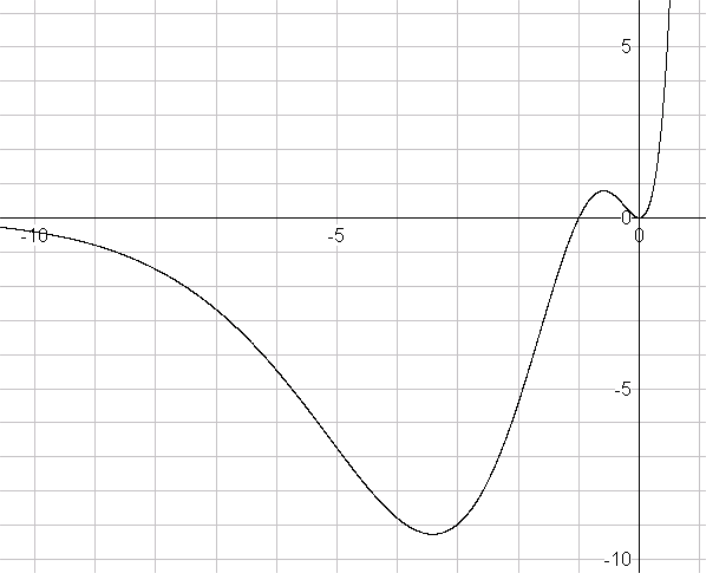
\includegraphics[width=12cm]{L4SZ2837}\end{center}%Use Desmos to check

	\Question Differentiate
\begin{tasks}(3)
	\task  $f (x) =\frac{1}{x^{2}}$ % $f^{ \prime } (x) = -2 x^{ -3} =\frac{ -2}{x^{3}}$
	\task $y =\sqrt[{3}]{x^{2}}$ %$f^{ \prime } \left (x\right ) =\frac{2}{3} x^{ -\frac{1}{3}} =\frac{2}{3 \sqrt[{3}]{x}}$ 
	\task $y =x^{5}$ % $y^{ \prime } =5 x^{4}$
	\task $y =\frac{1}{x^{3}}$ % $y^{ \prime } = -3 x^{ -4}$
	\task $y =x^{ -4}$ % $y^{ \prime } = -4 x^{ -5}$
	\task $y =x^{3/4}$ % $y^{ \prime } =\frac{3}{4} x^{ -\frac{1}{4}}$
	\task $y =\frac{1}{\sqrt{x}}$ % $y^{ \prime } = -\frac{1}{2} x^{ -\frac{3}{2}}$
\end{tasks}
\end{Exercise}
%---------------------------------------------
%--ANSWERS----First Principles----------------
%---------------------------------------------
\setboolean{firstanswerofthechapter}{true}
\begin{Answer}[ref={exFirstPrinciples}]
\Question %Find the derivative of the function 
\begin{tasks}
	\task  23
	\task -12
	\task 4
\end{tasks}

%\textbf{Graphing Exercises}\\	
\Question Use Desmos to plot the graph \\and compare to yours
\Question Use Desmos to check
\Question Use Desmos to check
\Question Use Desmos to check

\Question %Differentiate
\begin{tasks}
	\task $f^{ \prime } (x) = -2 x^{ -3} =\frac{ -2}{x^{3}}$
	\task $f^{ \prime } \left (x\right ) =\frac{2}{3} x^{ -\frac{1}{3}} =\frac{2}{3 \sqrt[{3}]{x}}$ 
	\task $y^{ \prime } =5 x^{4}$
	\task $y^{ \prime } = -3 x^{ -4}$
	\task $y^{ \prime } = -4 x^{ -5}$
	\task $y^{ \prime } =\frac{3}{4} x^{ -\frac{1}{4}}$
	\task $y^{ \prime } = -\frac{1}{2} x^{ -\frac{3}{2}}$
	
\end{tasks}
\end{Answer}%First Principles
\setboolean{firstanswerofthechapter}{false}
%-------------------------------------------------------------------
% QUESTIONS Standard Derivatives
%-------------------------------------------------------------------
\begin{Exercise}[title={Standard Derivatives},label=exStandardDerivatives]
	\Question Find $\frac{\text{dy}}{\text{dx}}$
	\begin{tasks}(2)
		\task $y =\frac{2}{5} x^{5}$ % $2 x^{4}$
		\task $y = -10$ % $0$
		\task $y = -3 x^{4}$ % $ -12 x^{3}$
		\task $y =\frac{2}{x^{4}}$ % $ -8 x^{ -5} =\frac{ -8}{x^{5}}$
		\task $y =\frac{1}{3 x^{3}}$ % $ -x^{ -4} =\frac{ -1}{x^{4}}$
	\end{tasks}
	
	\Question Differentiate
	\begin{tasks}(2)
		\task $f (t) =\sqrt{t}$ % $\frac{1}{2} t^{ -\frac{1}{2}} =\frac{1}{2 \sqrt{t}}$
		\task $f (t) =\sqrt{t^{3}}$ % $\frac{3}{2} t^{\frac{1}{2}} =\frac{3 \sqrt{t}}{2}$
		\task $f (z) =\sqrt[{3}]{z^{5}}$ % $\frac{5}{3} z^{\frac{2}{3}} =\frac{5 \sqrt[{3}]{z^{2}}}{3}$
		\task $f (x) =2 x^{3.2}$ % $6.4 x^{2.2}$ 
	\end{tasks}

	\Question Find the derivative
\begin{tasks}(2)
	\task $f (x) =2 x^{3} -3 x^{2} +4 x -1$ %$f^{ \prime } \left (x\right ) =6 x^{2} -6 x +4$
	\task $f (x) =x^{2} +x +1 +\frac{1}{x}$ %$f^{ \prime } \left (x\right ) =2 x +1 -\frac{1}{x^{2}}$ 
	\task $x^{8} +12 x^{5} -4 x^{4} +10 x^{3} -6 x +5$% $8 x^{7} +60 x^{4} -16 x^{3} +30 x^{2} -6$
\end{tasks}

\Question 
\begin{tasks}(2)
	\task Given $s =4 t^{2} -7 t +5$ find $\frac{d s}{d t}$ % $\frac{d s}{d t} =8 t -7$ 
	\task Find $\frac{d \left (3 x\right )}{d x}$  % $\frac{d \left (3 x\right )}{d x} =3$ 
	\task Find $\frac{d \left (3 u^{4}\right )}{d u}$ % $\frac{d \left (3 u^{4}\right )}{d u} =12 u^{3}$ 
	\task Given $f (x) =2 x -3$ find $D f (x)$ % $D f \left (x\right ) =2$ 
	\task Given $f (x) =e^{x} -x$ find $f^{ \prime } (x)$. Sketch the graph. % $f^{ \prime } \left (x\right ) =e^{x} -1$
	\task Differentiate $f (x) =\left (3 x\right )^{3}$ %$f^{ \prime } \left (x\right ) =81 x^{2}$
	\task Differentiate $g (x) =\left (x^{3}\right )^{5}$ %$g^{ \prime } \left (x\right ) =15 x^{14}$
	\task Find the derivative of $f (x) =e^{x} -x^{e}$ %$f^{ \prime } \left (x\right ) =e^{x} -e x^{e -1}$ 
\end{tasks}

	\Question Find the derived function
\begin{tasks}(2)
	\task $f (x) =\frac{1}{x^{3}} -\frac{1}{\sqrt[{4}]{x^{3}}}$ % $f^{ \prime } \left (x\right ) = -3 x^{ -4} +\frac{3}{4} x^{ -1\frac{3}{4}} = -\frac{3}{x^{4}} +\frac{3}{4 \sqrt[{4}]{x^{7}}}$
	\task $f (x) =\frac{\sqrt{x} +\sqrt[{3}]{x}}{\sqrt[{4}]{x}}$ % $f^{ \prime } \left (x\right ) =\frac{1}{4} x^{ -\frac{3}{4}} +\frac{1}{12} x^{ -\frac{11}{12}} =\frac{1}{4 \sqrt[{4}]{x^{3}}} +\frac{1}{12 \sqrt[{12}]{x^{11}}}$ 
	\task $g (x) =e x^{2} +2 e^{x} +x e^{2} +x^{e^{2}}$ % $g^{ \prime } \left (x\right ) =2 e x +2 e^{x} +e^{2} +e^{2} x^{e^{2} -1}$
	\task $f (x) =\sqrt[{3}]{x} +\sqrt[{5}]{2}$ % $f^{ \prime } \left (x\right ) =\frac{1}{3} x^{ -\frac{2}{3}} =\frac{1}{3 \sqrt[{3}]{x^{2}}}$
\end{tasks}

\Question Sketch the graphs and label your axes in radians
	\begin{tasks}(2)
	\task $f^{ \prime } (x)$ where $f (x) =\sin  x$ % Check with Desmos
	\task $g^{ \prime } (x)$ where $g (x) =\cos  x$  % Check with Desmos
	\task $h^{ \prime } (x)$ where $h (x)  =\tan x$  % Check with Desmos
\end{tasks}

\Question Differentiate the trigonometric functions
\begin{tasks}(2)
	\task $y =x^{2} \sin  x$ % $x^{2} \cos  x +2 x \sin  x$
	\task $f (x) =\sqrt{x} \sin  x$ % $\sqrt{x} \cos  x +\frac{1}{2 \sqrt{x}} \sin  x$
	\task $h (x) =\tan  (5 x)$ % $5 \sec ^{2} 5 x$
	\task $y =\frac{x}{\cos  x}$ % $\frac{\cos  x +x \sin  x}{\cos ^{2} x}$ 
	\task $g (t) =\cos  (\omega  t +\delta )$ % $ -\omega  \sin  \left (\omega  t +\delta \right )$ 
\end{tasks}

\Question Find the tangent line to the curve $y =e^{x} \cos  x$ at the point $(0 ,1)$. % $y -x -1 =0$ 
\Question A ladder $10 \mbox{m}$ long rests against a vertical wall. Let $\theta $ be the angle between the top of the ladder and the wall and let $x$ be the distance between the bottom of the ladder and the wall. If the bottom of the ladder slides away from the wall, how fast is $x$ changing with respect to $\theta $ when $\theta  =\frac{\pi }{3}$? % $\frac{d x}{d \theta } =5 \mathrm{m}/\mbox{rad}$

	\Question Find the derivative
\begin{tasks}(3)
	\task  $\sin  4 x$ % $4 \cos  4 x$
	\task $\frac{2}{\pi } \sin  \pi  x$ % $2 \cos  \pi  x$ 
	\task $5 \cos  3 x$ % $ -15 \sin  3 x$ 
	\task $\tan  3 x$ 	% $3 \sec ^{2} 3 x$ 
	\task $3 \tan  \left (x +2\right )$  %  $3 \sec ^{2} \left (x +2\right )$ 
	\task $\sin ^{3} x$ % $3 \sin ^{2} x \cos  x$ 
	\task $\sin ^{2} 3 x$ % $6 \sin  3 x \cos  3 x$ 
	\task $\sin ^{3} \left (x -1\right )^{2}$ % $6 \left (x -1\right ) \sin ^{2} \left (x -1\right )^{2} \cos  \left (x -1\right )^{2}$ 
	\task $\tan ^{2} 2 x$ %$4 \tan  2 x \sec ^{2} 2 x$
	
\end{tasks}

\end{Exercise}
%---------------------------------------------
%--ANSWERS----Standard Derivatives------------
%---------------------------------------------
\begin{Answer}[ref={exStandardDerivatives}]
	\Question %Find $\frac{\text{dy}}{\text{dx}}$
\begin{tasks}
	\task $2 x^{4}$
	\task $0$
	\task $ -12 x^{3}$
	\task $ -8 x^{ -5} =\frac{ -8}{x^{5}}$
	\task $ -x^{ -4} =\frac{ -1}{x^{4}}$
\end{tasks}

\Question %Differentiate
\begin{tasks}
	\task $\frac{1}{2} t^{ -\frac{1}{2}} =\frac{1}{2 \sqrt{t}}$
	\task $\frac{3}{2} t^{\frac{1}{2}} =\frac{3 \sqrt{t}}{2}$
	\task $\frac{5}{3} z^{\frac{2}{3}} =\frac{5 \sqrt[{3}]{z^{2}}}{3}$
	\task $6.4 x^{2.2}$ 
\end{tasks}

\Question %Find the derivative
\begin{tasks}
	\task $f^{ \prime } \left (x\right ) =6 x^{2} -6 x +4$
	\task $f^{ \prime } \left (x\right ) =2 x +1 -\frac{1}{x^{2}}$ 
	\task $8 x^{7} +60 x^{4} -16 x^{3} +30 x^{2} -6$
\end{tasks}

\Question 
\begin{tasks}
	\task $\frac{d s}{d t} =8 t -7$ 
	\task $\frac{d \left (3 x\right )}{d x} =3$ 
	\task $\frac{d \left (3 u^{4}\right )}{d u} =12 u^{3}$ 
	\task $D f \left (x\right ) =2$ 
	\task $f^{ \prime } \left (x\right ) =e^{x} -1$
	\task $f^{ \prime } \left (x\right ) =81 x^{2}$
	\task $g^{ \prime } \left (x\right ) =15 x^{14}$
	\task $f^{ \prime } \left (x\right ) =e^{x} -e x^{e -1}$ 
\end{tasks}

\Question %Find the derived function
\begin{tasks}
	\task $f^{ \prime } \left (x\right ) = -3 x^{ -4} +\frac{3}{4} x^{ -1\frac{3}{4}}\\
	 = -\frac{3}{x^{4}} +\frac{3}{4 \sqrt[{4}]{x^{7}}}$
	\task $f^{ \prime } \left (x\right ) =\frac{1}{4} x^{ -\frac{3}{4}} +\frac{1}{12} x^{ -\frac{11}{12}}\\ =\frac{1}{4 \sqrt[{4}]{x^{3}}} +\frac{1}{12 \sqrt[{12}]{x^{11}}}$ 
	\task $g^{ \prime } \left (x\right ) =2 e x +2 e^{x} +e^{2} +e^{2} x^{e^{2} -1}$
	\task $f^{ \prime } \left (x\right ) =\frac{1}{3} x^{ -\frac{2}{3}} =\frac{1}{3 \sqrt[{3}]{x^{2}}}$
\end{tasks}

\Question %Sketch the graphs and label your axes in radians
Check with Desmos\\
$\phantom{1}$\\
%$\phantom{1}$\\
\Question %Differentiate the trigonometric functions
\begin{tasks}
	\task $x^{2} \cos  x +2 x \sin  x$
	\task $\sqrt{x} \cos  x +\frac{1}{2 \sqrt{x}} \sin  x$
	\task $5 \sec ^{2} 5 x$
	\task $\frac{\cos  x +x \sin  x}{\cos ^{2} x}$ 
	\task $ -\omega  \sin  \left (\omega  t +\delta \right )$ 
\end{tasks}

\Question %Find the tangent line to the curve $y =e^{x} \cos  x$ at the point $(0 ,1)$. % 
$y -x -1 =0$ 
\Question %A ladder $10 \mbox{m}$ long rests against a vertical wall. 
$\frac{d x}{d \theta } =5 \mathrm{m}/\mbox{rad}$

\Question %Find the derivative
\begin{tasks}
	\task $4 \cos  4 x$
	\task $2 \cos  \pi  x$ 
	\task $ -15 \sin  3 x$ 
	\task $3 \sec ^{2} 3 x$ 
	\task $3 \sec ^{2} \left (x +2\right )$ 
	\task $3 \sin ^{2} x \cos  x$ 
	\task $6 \sin  3 x \cos  3 x$ 
	\task $6 \left (x -1\right ) \sin ^{2} \left (x -1\right )^{2} \cos  \left (x -1\right )^{2}$ 
	\task $4 \tan  2 x \sec ^{2} 2 x$
\end{tasks}	
\end{Answer}%Standard Derivatives

%-------------------------------------------------------------------
% QUESTIONS min, max, & tangents
%-------------------------------------------------------------------
\begin{Exercise}[title={Maximums, Minimums, and Tangents},label=exMinMax]
	\Question The function $y=7x-3$ has no turning point. Why? % $y=7x-3$ is a linear function and so has no maximum or minimum value. Its derivative is \emph{constant}.
	\Question Turning points are sometimes referred to as stationary points. Find the stationary points of the following functions:
	\begin{tasks}(3)
		\task $y=\frac{x^3}{3}-4x$ %$(2,0)$ and $(-2,0)$
		\task $y=x^2+\frac{16}{x}$ %$(2,12)$
		\task $f(x)=-x^4+4x^3-4x^2+1$ %$(0,1)$ and $(1,0)$ and $(2,1)$
	\end{tasks}
\Question Find the turning points and use the second derivative test to show if they are local maxima or local minima:
\begin{tasks}(2)
	\task $y=4-(3-x)^2$ %ans: $(3,4)$ is a local maximum
	\task $y=\frac{x^3}{3}-x$ %ans:$(-1,0.667)$ is a local maximum and $(1,-0.667)$ is a local minimum
	\task $f(x)=(3-x)(x+2)(x+5)$ %ans:$(-3.67,-14.82)$ min and $(1,36)$ max$
\end{tasks}
\Question Consider $f(x)=xe^x$. Do you think this function has a local max or min? Think of the graph of $y=e^x$. Plot the function using Desmos and find the turning point. %There is a local minimum at $(-1,-0.368)$. If you know how to use the product rule for differentiation you can find out without using desmos.
\Question Find the equations of the	tangent line and the normal line to the curve $y =x \sqrt{x}$ at the point $(1 ,1)$. % Tangent line is $2 y -3 x +1 =0$ \\\relax Normal line is $3 y +2 x -5 =0$ 
\Question Find the points on the curve $y =x^{4} -6 x^{2} +4$ where the tangent line is horizontal. %$\left (0 ,4\right ) ,\text{\quad \quad }\left (\sqrt{3} , -5\right ) ,\text{\quad \quad }\left ( -\sqrt{3} , -5\right )$
\Question At what point on the curve $y =e^{x}$ is the tangent line parallel to the line $y =2 x$? %$\left (\ln  2 ,2\right ) \approx \left (0.69 ,2\right )$
\Question Find a point $a$ on the curve $f (x) =x^{3} +2 x^{2} +3 x +4$ where $f^{ \prime } (a) =2$ % $a = -\frac{1}{3}$ or $ -1$
\Question Find where the tangent line to the function $f (x) =x^{3} -x +1$ is parallel to the line $y =x$.  % $x = \pm \sqrt{\frac{2}{3}}$ 

{\hspace{-0.6cm}\textbf{Graphing Exercise}}
\Question If $f (x) =2 x^{2} -x^{3}$ find $f^{ \prime }$, $f^{ \prime  \prime }$, $f^{ \prime  \prime  \prime }$, $f^{(4)}$. Use \Desmos to graph $f$, $f^{ \prime }$, $f^{ \prime  \prime }$, and $f^{ \prime  \prime  \prime }$ on a common screen. Describe whether these graphs are consistent with a geometric interpretation of these derivatives. %
\Question If $f (x) =\frac{1}{x}$ find $f^{ \prime } (x)$ and $f^{ \prime  \prime } (x)$ then graph $f$, $f^{ \prime }$and $f^{ \prime  \prime }$ on a common screen. Are your answers reasonable? %

\end{Exercise}
%---------------------------------------------
%--ANSWERS----min, max, & tangents------------
%---------------------------------------------
\begin{Answer}[ref={exMinMax}]
		\Question %The function $y=7x-3$ has no turning point. Why? % 
		$y=7x-3$ is a linear function and so has \\
		no maximum or minimum value. Its deriva-\\
		tive is \emph{constant}.
	\Question %Turning points are sometimes referred to as stationary points. Find the stationary points of the following functions:
	\begin{tasks}
		\task $(2,0)$ and $(-2,0)$
		\task $(2,12)$
		\task $(0,1)$ and $(1,0)$ and $(2,1)$
	\end{tasks}
	\Question %Find the turning points and use the second derivative test to show if they are local maxima or local minima:
	\begin{tasks}
		\task $(3,4)$ is a local maximum
		\task $(-1,0.667)$ is a local maximum and\\ $(1,-0.667)$ is a local minimum
		\task $(-3.67,-14.82)$ min and $(1,36)$ max
	\end{tasks}
	\Question %Consider $f(x)=xe^x$. Do you think this function has a local max or min? Think of the graph of $y=e^x$. Plot the function using Desmos and find the turning point. %
			  There is a local minimum at $(-1,-0.368)$\\
			  If you know how to use the product rule \\
			  for differentiation you can find out \\
			  without using desmos.
\Question %Find the equations of the tangent line and the normal line to the curve $y =x \sqrt{x}$ at the point $(1 ,1)$. %
Tangent line is $2 y -3 x +1 =0$ \\\relax Normal line is $3 y +2 x -5 =0$ 
\Question %Find the points on the curve $y =x^{4} -6 x^{2} +4$ where the tangent line is horizontal. %
$\left (0 ,4\right ) ,\text{\quad \quad }\left (\sqrt{3} , -5\right ) ,\text{\quad \quad }\left ( -\sqrt{3} , -5\right )$
\Question %At what point on the curve $y =e^{x}$ is the tangent line parallel to the line $y =2 x$? %
$\left (\ln  2 ,2\right ) \approx \left (0.69 ,2\right )$
\Question %Find a point $a$ on the curve $f (x) =x^{3} +2 x^{2} +3 x +4$ where $f^{ \prime } (a) =2$ % 
$a = -\frac{1}{3}$ or $ -1$
\Question %Find where the tangent line to the function $f (x) =x^{3} -x +1$ is parallel to the line $y =x$.  % 
$x = \pm \sqrt{\frac{2}{3}}$ 

%\textbf{Graphing Exercise}
\Question %If $f (x) =2 x^{2} -x^{3}$find $f^{ \prime }$, $f^{ \prime  \prime }$, $f^{ \prime  \prime  \prime }$, $f^{(4)}$. Use \Desmos to graph $f$, $f^{ \prime }$, $f^{ \prime  \prime }$, and $f^{ \prime  \prime  \prime }$ on a common screen. Describe whether these graphs are consistent with a geometric interpretation of these derivatives. %
See Desmos
\Question %If $f (x) =\frac{1}{x}$ find $f^{ \prime } (x)$ and $f^{ \prime  \prime } (x)$ then graph $f$, $f^{ \prime }$and $f^{ \prime  \prime }$ on a common screen. Are your answers reasonable? %
See Desmos	
\end{Answer}%min, max, & tangents

%-------------------------------------------------------------------
% QUESTIONS product, quotient, & chain rules
%-------------------------------------------------------------------
\begin{Exercise}[title={Product, Quotient, \& Chain Rules},label=exPQCRules]
	\Question Use the product rule to find the derivative
	\begin{tasks}(2)
		\task  $f (x) =x e^{x}$ % $f^{ \prime } \left (x\right ) =x e^{x} +e^{x} =e^{x} \left (x +1\right )$ 
		\task $g (x) =x^{2} e^{x}$ % $g^{ \prime } \left (x\right ) =x^{2} e^{x} +2 x e^{x} =x e^{x} \left (x +2\right )$ 
	\end{tasks}
	
	\Question Differentiate with respect to $x$ 
	\begin{tasks}(2)
		\task $x^{3} e^{x}$ % $\left (x^{3} e^{x}\right )^{ \prime } =x^{3} e^{x} +3 x^{2} e^{x} =x^{2} e^{x} \left (x +3\right )$
		\task $x^{ -3} e^{x}$ % $\left (x^{ -3} e^{x}\right )^{ \prime } =x^{ -3} e^{x} -3 x^{ -4} e^{x} =\frac{e^{x}}{x^{4}} \left (x -3\right )$ 
		\task $\left (x +1\right ) e^{x}$ % $\left (\left (x +1\right ) e^{x}\right )^{ \prime } =e^{x} \left (x +2\right )$
		\task $\left (x +2\right ) \left (x -2\right ) e^{x}$ % $\left (\left (x +2\right ) \left (x -2\right ) e^{x}\right )^{ \prime } =e^{x} \left (x^{2} +2 x -4\right )$
	\end{tasks}

	\Question Use the quotient rule to find the derivative
\begin{tasks}(2)
	\task  $y =\frac{3 x +1}{2 x -1}$ %$y^{ \prime } =\frac{ -5}{\left (2 x -1\right )^{2}}$ 
	\task $y =\frac{e^{x}}{x +1}$ % $y^{ \prime } =\frac{x e^{x}}{\left (x +1\right )^{2}}$ 
	\task $f (t) =\frac{2 t}{1 +t^{2}}$ find $\frac{d f}{d t}$ % $\frac{d f}{d t} =\frac{2 -2 t^{2}}{\left (1 +t^{2}\right )^{2}}$ 	
	\task $f (x) =\frac{A}{B +C e^{x}}$ % $f^{ \prime } \left (x\right ) =\frac{ -A C e^{x}}{\left (B +C e^{x}\right )^{2}}$ 
\end{tasks}

\Question Differentiate
\begin{tasks}(2)
	\task $\frac{3 x^{2}}{1 -x}$ % $\frac{ -3 x \left (x -2\right )}{\left (x -1\right )^{2}}$ 	
	\task $\frac{x}{x +2}$ % $\frac{2}{\left (x +1\right )^{2}}$ 	
	\task $\frac{\sqrt{x}}{x +2}$ % $\frac{2 -x}{2 \sqrt{x} \left (x +2\right )^{2}}$ 	
	\task $\frac{2 x^{2} +3 x +2}{e^{x}}$ % $\left (1 +x -2 x^{2}\right ) e^{ -x}$ 
		
\end{tasks}

{\hspace{-0.6cm}\textbf{Exercises involving Tangent and Normals}}
	\Question Find the equation of the tangent line and normal line to the curve $y =x e^{x}$ at the point $\left (0 ,0\right )$. %Tangent $y =x$\qquad Normal $y = -x$
	\Question The curve $y =1/(1 +x^{2})$ has the name witch of Maria Agnesi.
\begin{tasks}(1)
	\task  Find the equation of the tangent line to this curve at the point
	$\left (1 ,\frac{1}{2}\right )$.%$2 y +x -2 =0$
	\task  Use Desmos to draw the graph of the curve and the tangent line on the same grid.
\end{tasks}
	\Question The curve $y =x/(1 +x^{2})$ is called a serpentine. 
\begin{tasks}(1)
	\task  Find the equation of the tangent line at the point $\left (1 ,\frac{1}{2}\right )$.%Horizontal line $y =\frac{1}{2}$
	\task  Use Desmos to draw the graph of the curve and the tangent line on the same grid.
\end{tasks}

{\hspace{-0.6cm}\textbf{Composite Functions}}
\Question Let $f (x) =\sqrt{x}$ and $g (x) =x^{3}$ find $\left (f \circ g\right ) (x)$ and $\left (g \circ f\right ) \left (x\right )$. % $\left (f \circ g\right ) \left (x\right ) =\sqrt{x^{3}}\text{\quad \quad }\left (g \circ f\right ) \left (x\right ) =\left (\sqrt{x}\right )^{3}$
\Question Given $h \left (x\right ) =e^{x}$ and $j (x) =\frac{x^{2}}{2}$ find $\left (h \circ j\right ) (x)$ and $\left (j \circ h\right ) (x)$. % $\left (h \circ j\right ) \left (x\right ) =e^{\frac{x^{2}}{2}} =e^{x^{2}/2}\text{\quad \quad }\left (j \circ h\right ) \left (x\right ) =\frac{e^{2 x}}{2}$
	\Question The chain rule
\begin{tasks}(1)
	\task Find $F^{ \prime } (x)$ when $F (x) =\sqrt{1 +x^{2}}$. % $F^{ \prime } (x) =\frac{x}{\sqrt{1 +x^{2}}}$ 
	\task Given $y =\left (1 -x^{2}\right )^{5}$ find $\frac{d y}{d x}$. %$\frac{d y}{d x} = -10 x \left (1 +x^{2}\right )^{4}$ 
	\task Find the derivative of $e^{x^{2}}$. %$\left (e^{x^{2}}\right )^{ \prime } =2 x e^{x^{2}}$ 
	\task Find the derived function for $e^{e^{x}}$. %$\left (e^{e^{x}}\right )^{ \prime } =e^{e^{x}} \cdot e^{x} =e^{e^{x} +x}$
\end{tasks}

	\Question Differentiate with respect to $x$
\begin{tasks}(2)
	\task $\left (3 x +2\right )^{3}$ %$9 \left (3 x +2\right )^{2}$
	\task $\left (5 x +3\right )^{\frac{3}{5}}$%$\frac{3}{\left (5 x +3\right )^{2/5}}$
	\task $\frac{1}{2 x +1}$%$\frac{ -2}{\left (2 x +1\right )^{2}}$ 
	\task $\frac{3}{\left (4 -x\right )^{3}}$ %$\frac{9}{\left (4 -x\right )^{4}}$ 	
	\task $\sqrt{2 x -5}$ %$\frac{1}{\sqrt{2 x -5}}$ 
	\task $\sqrt[{3}]{5 -x^{2}}$%$\frac{ -2}{3 \sqrt[{3}]{\left (5 -x^{2}\right )^{2}}}$ 	
	\task $\frac{1}{\sqrt{x +2}}$ %$\frac{ -1}{2 \sqrt{\left (x +2\right )^{3}}}$ 	
	\task $e^{2 x^{3}}$ %$6 x^{2} e^{2 x^{3}}$ 
\end{tasks}

\Question You may have to combine rules to differentiate the following
\begin{tasks}(2)
	\task  $y =x^{2} e^{ -2 x}$ % $2 x e^{ -2 x} \left (1 -x\right )$
	\task $\left (1 -2 x\right )^{2} e^{ -x}$  % $ -e^{ -x} (1 -2 x) \left (5 -2 x\right )$ 
	\task $\frac{p +1}{\sqrt{p^{2} +1}}$ %  $\frac{1 -p}{\left (p^{2} +1\right ) \sqrt{p^{2} +1}}$
	\task $\left (x^{2} +3\right )^{2} \left (x -4\right )$ %$\left (x^{2} +3\right ) \left (5 x^{2} -16 x +3\right )$ 
	\task  $\left (x -3\right )^{3} \left (x +2\right )$  % $\left (x -3\right )^{2} \left (2 x -1\right )$ 
	\task $\sqrt{x +1} \left (x -1\right )^{2}$ % $\frac{\left (x -1\right ) \left (5 x +3\right )}{2 \sqrt{x +1}}$ 
	\task $e^{x^{2}} \sqrt{x +1}$ % $\frac{e^{x^{2}} \left (2 x +1\right )^{2}}{2 \sqrt{x +1}}$ 
	\task $\frac{x^{2} +x +2}{\left (x +1\right )^{2}}$ % $\frac{x -3}{\left (x +1\right )^{3}}$
\end{tasks}

\end{Exercise}
%---------------------------------------------
%--ANSWERS--product, quotient, & chain rules--
%---------------------------------------------
\begin{Answer}[ref={exPQCRules}]
	\Question %Use the product rule to find the derivative
\begin{tasks}
	\task $f^{ \prime } \left (x\right ) =x e^{x} +e^{x} =e^{x} \left (x +1\right )$ 
	\task $g^{ \prime } \left (x\right ) =x^{2} e^{x} +2 x e^{x} =x e^{x} \left (x +2\right )$ 
\end{tasks}

\Question %Differentiate with respect to $x$ 
\begin{tasks}
	\task $\left (x^{3} e^{x}\right )^{ \prime } =x^{3} e^{x} +3 x^{2} e^{x} =x^{2} e^{x} \left (x +3\right )$
	\task $\left (x^{ -3} e^{x}\right )^{ \prime } =x^{ -3} e^{x} -3 x^{ -4} e^{x}\\
	 =\frac{e^{x}}{x^{4}} \left (x -3\right )$ 
	\task $\left (\left (x +1\right ) e^{x}\right )^{ \prime } =e^{x} \left (x +2\right )$
	\task $\left (\left (x +2\right ) \left (x -2\right ) e^{x}\right )^{ \prime } =e^{x} \left (x^{2} +2 x -4\right )$
\end{tasks}

\Question %Use the quotient rule to find the derivative
\begin{tasks}
	\task $y^{ \prime } =\frac{ -5}{\left (2 x -1\right )^{2}}$ 
	\task $y^{ \prime } =\frac{x e^{x}}{\left (x +1\right )^{2}}$ 
	\task $\frac{d f}{d t} =\frac{2 -2 t^{2}}{\left (1 +t^{2}\right )^{2}}$ 
	\task $f^{ \prime } \left (x\right ) =\frac{ -A C e^{x}}{\left (B +C e^{x}\right )^{2}}$ 
\end{tasks}

\Question %Differentiate
\begin{tasks}
	\task $\frac{ -3 x \left (x -2\right )}{\left (x -1\right )^{2}}$ 
	\task $\frac{2}{\left (x +1\right )^{2}}$	
	\task $\frac{2 -x}{2 \sqrt{x} \left (x +2\right )^{2}}$ 
	\task $\left (1 +x -2 x^{2}\right ) e^{ -x}$ 
\end{tasks}

%\textbf{Exercises involving Tangent and Normals}
\Question %Find the equation of the tangent line and normal line to the curve $y =x e^{x}$ at the point $\left (0 ,0\right )$ %
Tangent $y =x$\qquad Normal $y = -x$
\Question %The curve $y =1/(1 +x^{2})$ has the name \textbf{witch of Maria Agnesi.}
\begin{tasks}
	\task  %Find the equation of the tangent line to this curve at the point
	$2 y +x -2 =0$
	\task  %Use Desmos to draw the graph of the curve and the tangent line on the same grid.
\end{tasks}
\Question %The curve $y =x/(1 +x^{2})$ is called a \textbf{serpentine}. 
\begin{tasks}
	\task  %Find the equation of the tangent line at the point $\left (1 ,\frac{1}{2}\right )$.%
	Horizontal line $y =\frac{1}{2}$
	\task  %Use Desmos to draw the graph of the curve and the tangent line on the same grid.
\end{tasks}

%\textbf{Composite Functions}
\Question $\left (f \circ g\right ) \left (x\right ) =\sqrt{x^{3}}\\
\left (g \circ f\right ) \left (x\right ) =\left (\sqrt{x}\right )^{3}$
\Question $\left (h \circ j\right ) \left (x\right ) =e^{\frac{x^{2}}{2}} =e^{x^{2}/2}\\
\left (j \circ h\right ) \left (x\right ) =\frac{e^{2 x}}{2}$
\Question %The chain rule
\begin{tasks}
	\task $F^{ \prime } (x) =\frac{x}{\sqrt{1 +x^{2}}}$ 
	\task $\frac{d y}{d x} = -10 x \left (1 +x^{2}\right )^{4}$ 	
	\task $\left (e^{x^{2}}\right )^{ \prime } =2 x e^{x^{2}}$ 
	\task $\left (e^{e^{x}}\right )^{ \prime } =e^{e^{x}} \cdot e^{x} =e^{e^{x} +x}$
\end{tasks}

\Question %Differentiate with respect to $x$
\begin{tasks}
	\task $9 \left (3 x +2\right )^{2}$
	\task $\frac{3}{\left (5 x +3\right )^{2/5}}$
	\task $\frac{ -2}{\left (2 x +1\right )^{2}}$ 
	\task $\frac{9}{\left (4 -x\right )^{4}}$ 	
	\task $\frac{1}{\sqrt{2 x -5}}$ 
	\task $\frac{ -2}{3 \sqrt[{3}]{\left (5 -x^{2}\right )^{2}}}$ 
	\task $\frac{ -1}{2 \sqrt{\left (x +2\right )^{3}}}$ 
	\task $6 x^{2} e^{2 x^{3}}$ 
\end{tasks}

\Question %You may have to combine rules to differentiate the following
\begin{tasks}
	\task $2 x e^{ -2 x} \left (1 -x\right )$
	\task $ -e^{ -x} (1 -2 x) \left (5 -2 x\right )$ 
	\task $\frac{1 -p}{\left (p^{2} +1\right ) \sqrt{p^{2} +1}}$
	\task $\left (x^{2} +3\right ) \left (5 x^{2} -16 x +3\right )$ 
	\task $\left (x -3\right )^{2} \left (2 x -1\right )$ 
	\task $\frac{\left (x -1\right ) \left (5 x +3\right )}{2 \sqrt{x +1}}$ 
	\task $\frac{e^{x^{2}} \left (2 x +1\right )^{2}}{2 \sqrt{x +1}}$ 
	\task $\frac{x -3}{\left (x +1\right )^{3}}$
\end{tasks}	
\end{Answer}%product, quotient, & chain rules

%-------------------------------------------------------------------
% QUESTIONS parametric differentiation
%-------------------------------------------------------------------
\begin{Exercise}[title={Parametric Differentiation},label=exParametric]
	\Question Use \desmos to sketch the parametric curves
	\begin{tasks}(2)
		\task $x =t^{2} -2 t$ and $y =t +1$ where $0 \leqslant t \leqslant 4$ % Check with desmos
		\task $x =\cos  t$ and $y =\sin  t$ where $0 \leqslant t \leqslant 2 \pi $ %
		\task $x =2 \cos  t$ and $y =\sin  t$ for $0 \leqslant t \leqslant 2 \pi $%
		\task $x =\cos  t$ and $y =\sin  2 t$ where $0 \leqslant t \leqslant 2 \pi $ %
		\task* $x =1.5 \cos  t -\cos  40 t$ and $y =1.5 \sin  t -\sin  40 t$ where $0 \leqslant t \leqslant 2 \pi $%
	\end{tasks}
	
	\Question Given $y =2 t$ and $x =t^{2}$ 
	\begin{tasks}
		\task Find $\frac{d y}{d x}$.% $\frac{d y}{d x} =\frac{1}{t}$
		\task By finding the appropriate value of $t$ show that $(1 ,2)$ lies on the parametric curve. % Let $t =1$
		\task Find the equation of the tangent line to the parametric curve at $(1 ,2)$. %$y -x-1 =0$
	\end{tasks}

	\Question Given
	$x =\cos  t$ and $y =\sin  t$ find the equation of the tangent line at the point $\left (\frac{\sqrt{2}}{2} ,\frac{\sqrt{2}}{2}\right )$. Where does this curve	have horizontal or vertical tangent lines? % $y +x =\sqrt{2}\text{,}$ Horizontal when $t =\frac{\pi }{2}$ or $\frac{3 \pi }{2}\text{,}$ Vertical when $t =0$ or $\pi $ 
	
	\Question Given $x =\cos  t$ and $y =\sin  2 t$ find the equation of the tangent line at the point $\left (\frac{\sqrt{3}}{2} ,\frac{\sqrt{3}}{2}\right )$. Where does this curve have horizontal or vertical tangent lines? % $2 y +4 \sqrt{3} x =6 +\sqrt{3}\text{,}$ Horizontal when $t =\frac{\pi }{4}\text{,}$ $\frac{3 \pi }{4}\text{,}$ $\frac{5 \pi }{4}\text{,}$ $\frac{7 \pi }{4}$ Vertical when $t =0\text{,}$ $\pi $
	
		\Question Find $\frac{d y}{d x}$ in terms of the parameter 
	\begin{tasks}(2)
		\task  $x =t^{2} +t\text{\quad \quad }y =t^{3} -t^{2}$ %$\frac{t \left (3 t^{2} +1\right )}{2 t +1}$ 
		\task $x =e^{t} \cos  t\text{\quad \quad }y =e^{t} \sin  t$ %$\frac{\cos  t +\sin  t}{\cos  t -\sin  t}$
		\task $x =a t^{2}\text{\quad \quad }y =2 a t$ ($a$ is constant) %$\frac{1}{t}$ 
		\task $x =a \sin  \theta \text{\quad \quad }y =b \cos  \theta $ %$ -\frac{b}{a} \tan  \theta $ 
		\task $x =2 \sin  \theta \text{\quad \quad }y =\cos  2 \theta $ %$ -2 \sin  \theta $ because $\sin  2 \theta  =2 \sin  \theta  \cos  \theta $ 
		\task $x =a \left (\theta  -\sin  \theta \right )\text{\quad \quad }y =a \left (1 -\cos  \theta \right )$%$\frac{\sin  \theta }{1 -\cos  \theta }$ 
	\end{tasks}
	
\end{Exercise}
%---------------------------------------------
%--ANSWERS-----parametric differentiation-----
%---------------------------------------------
\begin{Answer}[ref={exParametric}]
\Question Check with desmos%Use \desmos to sketch the parametric curves
%\begin{tasks}
%	\task Check with desmos
%	\task Check with desmos
%	\task Check with desmos
%	\task Check with desmos
%	\task Check with desmos
%\end{tasks}

\Question %Given $y =2 t$ and $x =t^{2}$ 
\begin{tasks}
	\task $\frac{d y}{d x} =\frac{1}{t}$
	\task  Let $t =1$
	\task $y -x-1 =0$
\end{tasks}

\Question %Given $x =\cos  t$ and $y =\sin  t$ find the equation of the tangent line at the point $\left (\frac{\sqrt{2}}{2} ,\frac{\sqrt{2}}{2}\right )$. Where does this curve	have horizontal or vertical tangent lines? % 
$y +x =\sqrt{2}\text{,}$ horizontal when $t =\frac{\pi }{2}$ or $\frac{3 \pi }{2}\text{,}$ \\Vertical when $t =0$ or $\pi $ 

\Question %Given $x =\cos  t$ and $y =\sin  2 t$ find the equation of the tangent line at the point $\left (\frac{\sqrt{3}}{2} ,\frac{\sqrt{3}}{2}\right )$. Where does this curve have horizontal or vertical tangent lines? % 
$2 y +4 \sqrt{3} x =6 +\sqrt{3}\text{,}$ horizontal when \\
$t =\frac{\pi }{4}\text{,}$ $\frac{3 \pi }{4}\text{,}$
 $\frac{5 \pi }{4}\text{,}$ $\frac{7 \pi }{4}$ vertical when $t =0\text{,}$ $\pi $

\Question %Find $\frac{d y}{d x}$ in terms of the parameter 
\begin{tasks}
	\task $\frac{t \left (3 t^{2} +1\right )}{2 t +1}$ 
	\task $\frac{\cos  t +\sin  t}{\cos  t -\sin  t}$
	\task $\frac{1}{t}$ 
	\task $ -\frac{b}{a} \tan  \theta $ 
	\task $ -2 \sin  \theta $ because $\sin  2 \theta  =2 \sin  \theta  \cos  \theta $ 
	\task $\frac{\sin  \theta }{1 -\cos  \theta }$ 
\end{tasks}	
\end{Answer}%parametric differentiation

%-------------------------------------------------------------------
% QUESTIONS related rates
%-------------------------------------------------------------------
\begin{Exercise}[title={Related Rates},label=exRelatedRates]
	\Question If $V$ is the volume of a cube with edge length $x$ and the cube is expanding as time passes, find $\frac{d V}{d t}$ in terms of $\frac{d x}{d t}$. %$3 x^{2} \frac{d x}{d t}$
	\Question Each side of a square is increasing at a rate of $6 \mbox{cm}$/$\mbox{s}$. At what rate is the area of	the square increasing when the area of the square is $16 cm^{2}$?  % $\frac{d A}{d t} =48 cm^{2}/\mbox{s}$ 
	\Question 
	\begin{tasks}(1)
		\task  If $A$ is the area of a circle with radius $r$ and the circle expands as time passes find $\frac{d A}{d t}$ in terms of $\frac{d r}{d t}$. %$ \frac{dA}{dt} =$\frac{dr}{dt}\cdot $\frac{dA}{dr}$$
		\task  Suppose oil spills from a ruptured tanker and spreads in a circular pattern. If the radius of the oil spill increases at a constant rate of $1 \mathrm{m}/\mbox{s}$ how fast is the area of the spill increasing when the radius is $30 \mbox{m}$? % $\frac{d A}{d t} =60 \pi  \mathrm{m}/\mbox{s}$
	\end{tasks}
	
	\Question If a snowball melts so that its surface area decreases at a rate of $1 cm^{2}$/$\mbox{min}$, find the rate at which the diameter decreases when the diameter is $10$ $\mbox{cm}$. The following steps may help you to solve this problem. %$ -\frac{1}{20 \pi }$ \\\relax decreasing at a rate of $\frac{1}{20 \pi } cm/\mbox{min}$
	\begin{tasks}[counter-format=(tsk[r])](1)
		\task What quantities are given in the problem? 
		\task What is the unknown?
		\task Draw a picture of the situation for any time $t$. 
		\task Write an equation that relates the quantities. 
		\task Solve for the unknown quantities.		
	\end{tasks}
	\Question At noon ship A is $150 \mbox{km}$ west of a ship B. Ship A is sailing east at $35 \mbox{km}$/$\mbox{h}$ and ship B is sailing north at $25 \mbox{km}$/$\mbox{h}$. How fast is the distance between the ships changing at 4:00 P.M.? %$\frac{215}{\sqrt{101}} \approx 21.4 \mathrm{m}/\mbox{h}$ 
	\Question A plane flying horizontally at an altitude of $2 \mbox{km}$ and a speed of $800 km/\mbox{h}$ passes directly over a radar station. Find the rate at which the distance from the plane to the station is increasing when it is $3 \mbox{km}$ away from the station.%$\frac{800 \sqrt{5}}{3} \approx 596.3 km/\mbox{h}$


\end{Exercise}
%---------------------------------------------
%--ANSWERS----- related rates-----------------
%---------------------------------------------
\begin{Answer}[ref={exRelatedRates}]
	\Question %If $V$ is the volume of a cube with edge length $x$ and the cube is expanding as time passes, find $\frac{d V}{d t}$ in terms of $\frac{d x}{d t}$ %
	$3 x^{2} \frac{d x}{d t}$
\Question %Each side of a square is increasing at a rate of $6 \mbox{cm}$/$\mbox{s}$. At what rate is the area of	the square increasing when the area of the square is $16 cm^{2}$?  % 
$\frac{d A}{d t} =48$ cm$^2$/s 
\Question 
\begin{tasks}
	\task  %If $A$ is the area of a circle with radius $r$ and the circle expands as time passes find $\frac{d A}{d t}$ in terms of $\frac{d r}{d t}$ %
	$ \frac{dA}{dt} =\frac{dr}{dt}\cdot \frac{dA}{dr}$
	\task  %Suppose oil spills from a ruptured tanker and spreads in a circular pattern. If the radius of the oil spill increases at a constant rate of $1 \mathrm{m}/\mbox{s}$ how fast is the area of the spill increasing when the radius is $30 \mbox{m}$? % 
	$\frac{d A}{d t} =60 \pi$ m$^2$s$^{-1}$
\end{tasks}

\Question %If a snowball melts so that its surface area decreases at a rate of $1 cm^{2}$/$\mbox{min}$, find the rate at which the diameter decreases when the diameter is $10$ $\mbox{cm}$. You should use the following steps to solve this problem. %
$\frac{-1}{20 \pi }$ decreasing at a rate of $\frac{1}{20 \pi }$ cm/min 
\Question %At noon ship A is $150 \mbox{km}$ west of a ship B. Ship A is sailing east at $35 \mbox{km}$/$\mbox{h}$ and ship B is sailing north at $25 \mbox{km}$/$\mbox{h}$. How fast is the distance between the ships changing at 4:00 P.M.? %
$\frac{215}{\sqrt{101}} \approx 21.4$ km/h 
\Question %A plane flying horizontally at an altitude of $2 \mbox{km}$ and a speed of $800 km/\mbox{h}$ passes directly over a radar station. Find the rate at which the distance from the plane to the station is increasing when it is $3 \mbox{km}$ away from the station.%
$666$ km/h	
\end{Answer}% related rates

%-------------------------------------------------------------------
% QUESTIONS Optimisation
%-------------------------------------------------------------------
\begin{Exercise}[title={Optimisation},label=exOptimisation]
	\Question Divide $50$ into two parts such that the product of the two parts is a maximum. % $25$ and $25$
	\Question Find the number that exceeds its square by the greatest amount. %  $\frac{1}{2}$ 
	\Question A farmer has $2400 \mbox{m}$ of fencing and wants to fence off a rectangular field that borders a straight river. He needs no fence along the river. What are the dimensions of the field that has the greatest area? % $1200 \mbox{m}$ by $600 \mbox{m}$
	\Question A farmer wishes to fence off a corner of a field where there is an existing hedge on two sides. The hedge is to be used to fence the two sides. If he has $300 \mbox{m}$ of fencing available, find the dimensions $a$ and $b$ so that he encloses the maximum area.\\ 
	 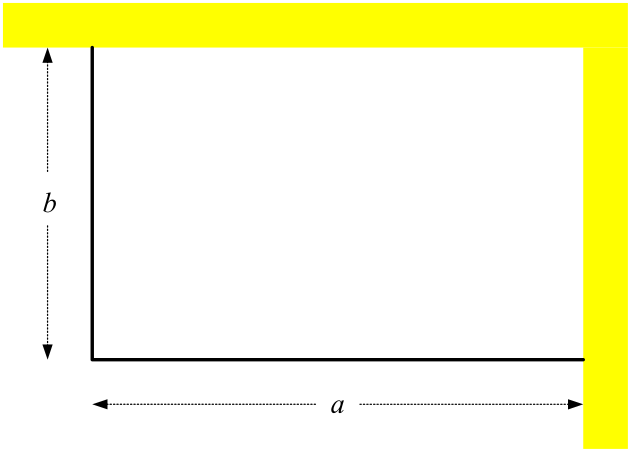
\includegraphics[ width=2.5711in, height=1.8498in,]{L4SZ2838}\\ % $150 \mbox{m}$ by $150 \mbox{m}$ 
	\Question The volume of the cone is given by the formula $V(r)= \frac{10\pi r^2}{3}-\frac{\pi r^3}{3}$. Find the radius of the cone at its maximum volume.%ans:$\frac{20}{3}$ cm
	\Question The total cost of holding a large event is composed of the venue hire, $V$, times the venue tax, $T$, plus the entertainment, $E$. These values can all be estimated based on the number of people attending the event, $p$, such that: $V(p)=50p+80$, $T(p)=0.002p-0.4$, and $E(p)=36000-60p$. Find the minimum cost.%ans:\$20032 for 399 people 
	\Question Find the area of the greatest rectangle that can be inscribed in a semicircle	of radius $r$. % Area $ =r^{2}$ 
	\Question If $1200 cm^{2}$ of material is available to make a box with a square base and an open top. Find the largest possible volume of the box. (Hint: There is no wasted material.) %Dimensions are 20 by 20 by 10, Volume $ =4000 cm^{3}$ 

\end{Exercise}
%---------------------------------------------
%--ANSWERS----- optimisation------------------
%---------------------------------------------
\begin{Answer}[ref={exOptimisation}]
\Question %Divide $50$ into two parts such that the product of the two parts is a maximum. % 
$25$ and $25$
\Question %Find the number that exceeds its square by the greatest amount. %  
$\frac{1}{2}$ 
\Question %A farmer has $2400 \mbox{m}$ of fencing and wants to fence off a rectangular field that borders a straight river. He needs no fence along the river. What are the dimensions of the field that has the greatest area? % 
$1200 \mbox{m}$ by $600 \mbox{m}$
\Question %A farmer wishes to fence off a corner of a field where there is an existing hedge on two sides. The hedge is to be used to fence the two sides. If he has $300 \mbox{m}$ of fencing available, find the dimensions $a$ and $b$ so that he encloses the maximum area.\\ 
%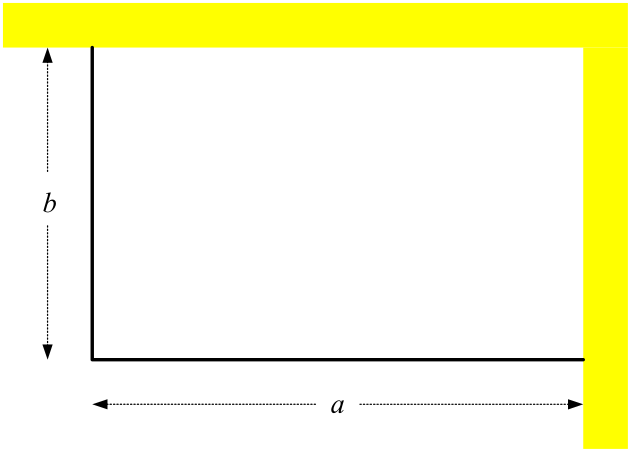
\includegraphics[ width=2.5711in, height=1.8498in,]{L4SZ2838}\\ % 
$150 \mbox{m}$ by $150 \mbox{m}$ 
\Question %The volume of the cone is given by the formula $V(r)= \frac{10\pi r^2}{3}-\frac{\pi r^3}{3}$. Find the radius of the cone at its maximum volume.%
$\frac{20}{3}$ cm
\Question %The total cost of holding a large event is composed of the venue hire, $V$, times the venue tax, $T$, plus the entertainment, $E$. These values can all be estimated based on the number of people attending the event, $p$, such that: $V(p)=50p+80$, $T(p)=0.002p-0.4$, and $E(p)=36000-60p$. Find the minimum cost.%
\$20,032.00 for 399 people
\Question %Find the area of the greatest rectangle that can be inscribed in a semicircle	of radius $r$. %
 Area $ =r^{2}$ 
\Question %If $1200 cm^{2}$ of material is available to make a box with a square base and an open top. Find the largest possible volume of the box. (Hint: There is no wasted material.) %
20 by 20 by 10, Volume $ =4000 cm^{3}$ 	
\end{Answer}% optimisation
